\documentclass{acm_proc_article-sp}
\usepackage{graphicx}
\usepackage{listings}
\usepackage{hyperref}

% definitions
\def \tool {InputFinder}  

\begin{document}

\title{InputFinder: Reverse Engineering Closed Binaries via Side Channels}
\numberofauthors{2}
\author{
\alignauthor
Bogdan Copos\\
	\affaddr{University of California, Davis}\\
	\email{bcopos@ucdavis.edu}
\alignauthor
Praveen Murthy\\
	\affaddr{Fujitsu Laboratories of America}\\
	\email{praveen.murthy@us.fujitsu.com}
}
\maketitle

\begin{abstract}
The effectiveness of many dynamic analysis techniques depends heavily on the completeness of the test suite applied during the analysis process.
Test suites are often composed by developers and aim at covering (and testing) all of the functionality of a software system.
However, test suites may not be complete, if they exist at all.
To date, only two methods exist for automatically generating test input for closed binaries: fuzzing and symbolic execution.
Despite previous success methods in identifying bugs, both techniques have limitations.
In this paper, we propose a new method for autonomously generating valid input and identifying protocols for closed x86 binaries.
To assess its effectiveness, we have developed \tool{} and tested it against binaries from the DARPA Cyber Grand Challenge example set.
Our evaluations show that ...
\end{abstract}

\section{Introduction}
%introduction
Software testing, particularly vulnerability testing, is an expensive and labor intensive process.
For many years, researchers have explored both static and dynamic methods for analyzing programs \cite{smartfuzzer}.
While static analysis is thought to be more thorough, dynamic testing is often preferred due to its time efficiency.
However, dynamic testing heavily depends on availability of input or test suites.

%motivation
Without complete test suites, the program cannot be properly tested and bugs may be omitted.
While valid input can be learned from software documentation or source code, when such information is not available or complete, other methods must be used.
Automated dynamic analysis techniques such as fuzzing and symbolic execution attempt to generate input for a given program.
Currently these are the only two options available and both approaches present discouraging limitations.

In this paper, we introduce a new method for generating valid user-input for closed binaries. 
Our method is composed of two main components.
The first component exploits side channels to build valid input for closed binaries.
Specifically, as the program is given various input, \tool{} records the number of instructions retired during the program's execution for each input and compares the recorded value to learn the program's expected input.
The same side channel is used by \tool{} to also find the expected input size and to categorize the expect input based on type.
The second component uses the discovered input to build a protocol state machine associated with the tested program.
This enables the generation of a more thorough test suite.

The main contributions of this paper are as follows:
\begin{itemize}
	\item We introduce a new approach to automatically generate input valid strings for unknown, closed-source binaries by leveraging hardware instruction counters. Our method relies on observing changes in the number of instructions executed by programs during their input validation process to learn valid input strings.
	\item We describe how our method can be used to not only find valid input strings, but also to determine the expect input size and classify input based on type (e.g. alphabetic, alphanumeric, numeric, etc.).
	\item We develop a method for generating protocol state machines using the valid input previously found.
	\item We implement the techniques presented and evaluate the tool using binaries published by DARPA as part of the 2014 Cyber Grand Challenge competition \cite{darpacgc}. Additionally, we compare our approach to the manual process used by a security specialist to crack a binary as part of a job interview \cite{interviewbinary}.
\end{itemize}

The paper is organized as follows.
Section \ref{background} covers background information relating to concepts utilized in this work.
Section \ref{prevwork} discusses related works and highlights differences between the related works and the work presented here.
The details of our approach are explained in Section \ref{methodology}. First, the method for finding valid input is described. Then we introduce our method for building protocol state machines using the discovered input.
Section \ref{results} describes evaluation of the work presented and the results.
In Section \ref{futurework}, we share future plans for our work and explain cases which the proposed method does not handle.


\section{Background} \label{background}
\subsection{Side Channels} \label{bg_sidechannels}
Side channels are streams of information that can be retrieved from the hardware of a device running a given program.
This information can be used to learn gather knowledge regarding the program's internal components.
Side channels have been widely explored by security researchers in order to discover weaknesses in programs \cite{weinbergside, schindler2002combined, genkin2014rsa, genkinstealing}.
In cryptography, side channel attacks exploit such information channels to defeat crypto systems \cite{zhou2005side, black2002black, okeya2006side}.
Recently, side channel attacks, such as OpenSSL's CREAM cache timing attack have made headlines \cite{creamssl}.
Similar to CREAM and other side channel attacks, the technique discussed in this paper exploits such information channels to generate valid input for binaries.
\subsection{Hardware counter registers} \label{bg_hardwarereg}
Most modern microprocessors have a set of special-purpose registers used to count hardware events.
Each register, or counter, can be programmed to measure specific events such as cache misses, floating point operations, and even instructions executed.
Such hardware performance counters are often used by software developers to analyze their programs and improve on running time and efficiency.
However, in this paper we show how such performance counters can also be exploited as side channels.
Utilities, such as Linux/Unix `perf', take advantage of such hardware counters in order to provide developers with useful information about a program's performance.
`perf' allows developers to specify the desired hardware event they wish to measure.
Once events have been selected, `perf' interacts with the appropriate kernel modules to program the hardware counters accordingly.
In this work, we use `perf' to count the number of \textbf{user-land} instructions executed as a program is tested with various input.
While other options are available for counting instructions executed, we chose `perf' for its efficiency and minimal overhead.
The number of \textit{total} instructions retired oscillates significantly for a binary from execution to execution.
This phenomena reflects fluctuations in instructions executed by the kernel depending on the state of the machine due to cache-misses and other factors.
Since we rely on this count, such variations are problematic.
However, experimentally, the number of \textit{user-land} instructions only varies, on average, by one instruction, giving us a reliable counter.
\subsection{Execution/Dynamic Matching} \label{bg_dynamicsim}
In many application areas, including clone detection and software debugging, there is a need for comparing executions of a program (or multiple versions of a program).
One of the proposed approaches aimed at tackling this issue is dynamic matching.
Dynamic matching works by first collecting execution traces of different executions.
Such traces can be collected through a number of ways.
One option includes the use of Pin \cite{pintool}.
Pin is a framework for building customized binary analysis tools and can be used to design a tool which creates a transcript of the instructions executed by a program.
Once the traces are collected, they are analyze and mappings between instructions of different executions are produced.
These mappings can be used to understand the relationship between two executions (or two versions of a program).
In this work, we rely on the concept of dynamic matching and the Pin framework to develop a protocol state machine generator for closed binaries.


\section{Previous Work} \label{prevwork}
Dynamic analysis has been extensively studied in academia and is used widely in the industry by security specialists.
Two of the main approaches to vulnerability testing are fuzzing and symbolic execution.

Fuzzers are a popular choice amongst software testers.
They are easy to use, easy to implement, and have produced surprising results in the past \cite{millerfuzz, millerfuzzrevisited}.
There are two classes of fuzzers: black box fuzzers and white box fuzzers.
In black box fuzzing, the program is watched as it is tested with randomly generated input.
If the program crashes, the input(s) are recorded and reported.
No prior program specifications or knowledge of the input format is available in such cases.
Since black box fuzzing is completely random, its effectiveness is limited, especially with respect to coverage.
On the other hand, in white box fuzzing, inputs are used to gather symbolic constraints which are in turn systematically negated and solved to produce more inputs.
The approach introduced in this paper is similar to white box fuzzing in that information from the program's execution is used to craft valid input.
White box fuzzing differs from black box fuzzing in that it uses the program's feedback to make inferences about valid input and use constraint solvers to generate more input.
White box fuzzing can attain better code coverage but can be slow and is crippled by innate limitations of constraint solvers.

One of the works utilizing white box fuzzing is \cite{molnar2009dynamic} which introduces SmartFuzz, a dynamic test generation tool.
SmartFuzz uses symbolic execution to learn about the program's input and passes that information to a fuzzer for test case generation.
The main difference between our work and SmartFuzz is that our work does not use symbolic execution to gain insight into the format of the input.
Similar to SmartFuzz, the output of our work can be used by a fuzzer to generate test cases.

Another related work is presented in \cite{smartfuzzer}, where the authors use a combination of static and dynamic analysis to build a smart fuzzer.
Their work uses static analysis to collect preliminary information such as an approximation of the inter procedural control flow graph.
Having gathered static information, their dynamic analysis engine executes the program while monitoring dependencies between the input and the dynamic control flow path experienced by the program.
Their work also takes advantage of a constraint solver that given a path of the program generates input which forces the program to follow the chosen path.
Our work \tool{} differs from \cite{smartfuzzer} in several ways.
One difference is that our work uses neither static analysis nor constraint solvers.
Instead we rely only on information extracted from the execution of the program. 

Symbolic execution is another method used for generating valid input.
In symbolic execution, an interpreter gathers constraints related to input throughout the program's execution, rather than using the provided input.
At the end of the execution, a constraint solver takes the constraints gathered and outputs valid program input.
Symbolic execution has been proven effective by previous works \cite{symbolicexecution, exesymex}.
Similar to white box fuzzing, symbolic execution has a fundamental limitation with respect to constraint solving.
While symbolic execution engines perform well with linear constraints, non-linear constraints greatly impact efficiency.
One of the most important works in this area is described in \cite{exesymex} which introduces EXE, a dynamic analysis tool capable of generating inputs that crash programs by running the programs with symbolic input.
Unlike symbolic execution, the approach presented in our work is not hindered by constraint solvers and does not require any instrumentation or source code.
\tool{} does not execute the program with symbolic input but rather it uses concolic input and information about the execution of the program to craft valid input.

There have also been numerous works studying and applying dynamic similarity.
In \cite{blanketexec}, the authors propose blanket execution, a novel dynamic equivalence testing technique.
Blanket execution is designed to collect information about the execution of functions, including side effects, which is then used for similarity testing.
Both our approach and blanket execution use a dynamic approach to gather information about the program.
However, our approach aims at finding similarities in executions of entire programs (not just functions) with various inputs.
This allows us to discover differences in inputs which experience different control flow paths.

Another area of research relevant to this paper is protocol reverse engineering.
An important result in this area is \cite{prospex} which introduces a technique for extracting protocol specifications from packet captures and automatically generating input which can be used by a stateful fuzzer.
There are two notable difference between Prospex and our work.
While the end result is similar, \tool{} assumes no prior knowledge about the tested program and hence it does not utilize packet captures for protocol specification extraction.
Instead, \tool{} infers the protocol through dynamic analysis by automatically finding input and using that to generate a protocol state machine.
To date, there are no protocol reverse engineering techniques which assume no prior knowledge about the program's input.

\section{Methodology} \label{methodology}
% add some high level intro for both finding input and psm stuff
\tool{} is composed of two main modules.
The first module is responsible for discovering input and properties of the expected input, including input size and the type of the input.
The input can then be used by the second component to generate a protocol state machine, information which may then be used by a stateful fuzzer.
\subsection{Finding Valid Input}
The majority of software programs accept input, perform transformations on the input and output results.
However, most programs do not accept completely random input.
Input usually passes through an input validation filter.
Such filters are snippets of code responsible for distinguishing between valid or good input (i.e. input the program was constructed to understand and accept) and bad input (i.e. input which is not useful or does not follow the desired format).
Although validation mechanisms can be very sophisticated, they are often a combination of string comparisons and conditional statements.
Our method exploits changes in the number of user-land instructions retired during multiple executions with varying inputs to make inferences about the program's validation mechanism.
These changes reflect different execution paths of the program as a response to both valid and invalid input.
Assuming most input is invalid, our method observes differences in the number of instructions executed to detect input which passes the validation mechanism.

\begin{figure*}[t]
\centering
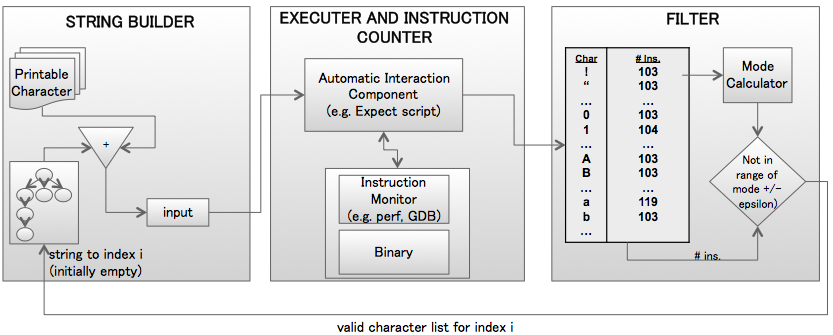
\includegraphics[height=2.5in,width=6.5in]{architecture.png}
\label{fig:architecture}
\caption{This figure depicts the architecture of the finding input process. There are three main parts: the execution engine, the valid character filter and the input string builder.}
\end{figure*}

Figure \ref{fig:architecture} shows the overall architecture of the finding input component of \tool{}.
The process is recursive and is composed of two steps.

\begin{lstlisting}[caption={Pseudocode implementing the input finding process},label={findinputcode},escapeinside={@}{@}]
string s = ""
find_input(s, results) {
    for char in printableChars:
    #record number of instr executed per input
    @\label{findinputcode_exec}@instrPerChar[char] = exec_bin_wperf(s+char)

    #calculate mode for all instr counts	
    @\label{findinputcode_mode}@mode = calculate_mode(instrPerChar)

    #filtering stage: identify valid chars
    for char in instrPerChar:
      count = instrPerChar[char]
      min = mode - epsilon
      max = mode - epsilon
      @\label{findinputcode_filter}@if not count in range(min, max):
	validCharsList.append(char)
	
    #base case
    if len(validCharsList) == 0:
       # reached end of input string
       results.put(s)
       return 0

    #continue crafting input strings	
    @\label{findinputcode_fork}@for valid_char in validCharsList:
      find_input(s+validChar, results)
}

\end{lstlisting}

The steps of the process for finding valid input are described in \autoref{findinputcode} and outlined below. Starting with an empty string, \textit{s}:
\begin{enumerate}
\item \tool{} executes the program once for every printable character and records the number of user-land instructions executed by the program with the given input. The input is a string concatenation of the string \textit{s} and the current printable character. The Unix `perf' utility is used for monitoring the number of instructions executed. Note that \tool{} does not record the total number of instructions but rather user-land instructions. The reason for this, as explained in Section \ref{bg_hardwarereg}, is that the total number of instructions executed can vary greatly from execution to execution due to operating system factors (e.g. branch prediction, cache). The Expect tool is used for automating the program interaction. This step is shown in line \autoref{findinputcode_exec} of \autoref{findinputcode}.
\item Once all executions have been completed (one for each character), the mode number of instructions retired is computed across all executions. The mode is defined as the value that appears most often in the set of recordings. This is done in line \autoref{findinputcode_mode} of \autoref{findinputcode}
\item Next is the filtering stage which is responsible for identifying characters likely to be part of a valid input string at the current index. Under the assumption that most characters are not valid for the current index, \tool{} gathers all characters with the number of instructions executed outside the range of the mode +/- an epsilon value, as shown in line \autoref{findinputcode_filter} of \autoref{findinputcode} . These characters represent valid characters for the current index of the input string. The epsilon value accounts for small variations in the hardware counters. While the initial reaction is to expect a valid character to result in more instructions executed than a non-valid character, this is not always the case. As discussed earlier, the input validation mechanism can be complex and can vary in behavior. The validation mechanism may verify input against all accepted input strings before denying the provided input. Such a scenario results in more instructions executed for invalid input than valid input.
\item For each valid character \textit{c}, \tool{} forks with every child process repeating steps 1-4, appending \textit{c} to the end of the string \textit{s} (starting at line \autoref{findinputcode_fork} of \autoref{findinputcode}). If no valid characters are found, the end of a valid input string has been reached and the string is recorded. If the current index is 0 and no valid characters have been found, the given binary has no predefined input commands.
\end{enumerate}

\begin{figure*}[t]
\centering
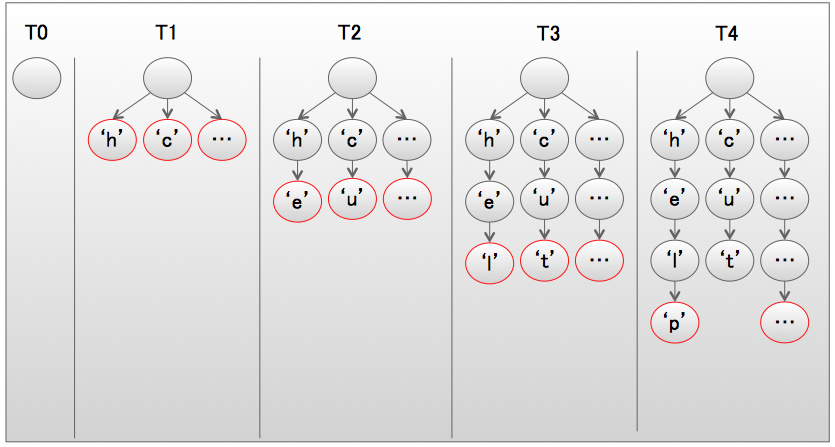
\includegraphics[height=2in,width=6.5in]{string_builder.png}
\label{fig:string_builder}
\caption{This diagram visualizes the input string being constructed throughout five consecutive time stages of the execution of \tool{}. Multiple outgoing arrows represent a process forking. This occurs when multiple valid characters are detected for a given index of the input string and, as a result, the finding input process forks to concurrently handle all of the discovered characters}
\end{figure*}

Figure~\ref{fig:string_builder} depicts the results of the above process over the span of five consecutive time stages.
As seen in the figure, at time \textit{T0}, \tool{} begins with an empty string.
At time \textit{T1}, \tool{} finds valid characters for index 0 of the input and is forked into \textit{n} child processes where \textit{n} is the number of valid characters found.
The process continues until all child processes are done.

\subsubsection{Finding Desired Input Size}
The same side channels can be used to detect the expected size of the program's input or even the program's input buffer.
Most programs are designed to read a predefined number of bytes from the source of input and store them in a buffer.
Depending on the implementation, when a program is given more input than the size of the buffer, additional instructions may be executed.
Regardless of the number of instructions executed, the behavior of the program changes.
A program may exit when the number of provided bytes is larger than expected.
Similarly, once the input buffer size limit has been reach, a program may check to see if the next byte is a newline or EOF.
Some methods, such as C's `fgets()' function, read character by character [EXPLAIN]
Our method observes such differences in the number of user-instructions retired as the program is given increasingly larger input.

To start, \tool{} finds the set of all invalid characters for index 0 of all input strings and picks one at random.
The character selected is used to build invalid input strings of various sizes.
It is crucial to use invalid input to avoid noisy fluctuations in the number of instructions executed due to valid input processing.
Initially, the program is executed with short length input strings (i.e. two and three characters).
The number of user-land instructions executed during these two executions are recorded.
These two values may be equal or differ, depending on the program's logic.
If the two values are equal [EQUAL]
The two values can also differ because... [DIFFERENT]

\subsubsection{Categorizing Input}
Our method is also capable of classifying the input discovered.
Generated input strings are classified in three categories: alphabetic, numeric, alphanumeric.
Similarly, the classification algorithm detects special characters.
Once enough input strings have been identified, \tool{} uses the categorization data to generalize about the type of input the program accepts.
Such information is valuable especially in cases where the inputs discovered are all numeric or contain (one or more) special characters.
Having learned such information about the program, the testing platform (e.g. fuzzer) can be adjusted to proceed accordingly.

\subsection{Generating Protocol State Machine}
% TODO
% add diagram depicting process
Thus far, we have described how \tool{} discovers valid input for a given binary autonomously.
However, some binaries have an implicit protocol.
Consider, for example, a database management program.
Without first selecting a database and perhaps even a table, some commands such as `insert' or `select' are useless and have no effect on any data.
This is where the second component of \tool{} steps in.
Specifically, this component identifies expected permutations of the discovered input strings.

\begin{lstlisting}[caption={Pseudocode implementing the protocol state machine generator},label={lst:psmcode}]
void main(inputs) {
  for len in len(inputs):
    permutations = get_permutation(len)
    results = []
    for p in permutations:
      exec(p, 0, results)
    compare_inputs(results, inputs)
}

void exec(cmds, i, results) {  
  i = 0

  # base case
  if i == len(cmds):
    results.append(cmds)
    return 0

  #finds args for input string at index i
  initCmds = cmds[0:i]
  cmd = cmds[i]
  args = find_args(initCmds, cmd, i)

  for arg in args:
    cmds[i] = cmds[i] + arg  #concatenation
    exec(cmds, i+1, results)
}
    
void compare_inputs(results, inputs) {
  #organize results
  for cmds in results:
    lastCmd = cmds[len(cmds)]
    
    trace = get_pin_trace(cmds)
    
    traceForLastCmd = split_trace(cmds)
    traceVector = dfs_cfg(trace) 
    
    traces[lastCmd][cmds] = traceVector
  
  #compare traces for same input/cmd
  # from different permutations
  for cmd in cmds:
    for cmdTraces in traces[cmd]:
      clusters = compare(cmdTraces)
   
   #find outliers in clusters
   filter(clusters)
}
		
\end{lstlisting}

Once input has been discovered, \tool{} constructs a protocol state machine.
The architecture of this component is depicted in Figure \ref{fig:XXXXpsm_arch}.
The process is describe below and shown as pseudocode in Listing \ref{lst:psmcode}.
First, all possible permutations of all sizes from 1 to the number of input strings discovered are computed.
Every permutation is passed through the dynamic analysis engine.
The dynamic analysis execution engine first splits the permutation into individual input strings.
Maintaining the original order of the inputs, the engine tests each string for the presence of expected arguments.
For example, if the input string is `SET' and the program accepts input of the format `SET data', the analysis tries to determine that `data' is a valid argument.
The arguments found are saved for later use.
Once every input pertaining to a permutation has been tested for arguments, the inputs are passed through a instrumented binary for the collection of execution trace.
The binary is instrumented with a Pin tool, developed by us, which logs the instructions executed as a function of time.
Once all permutations of a given size have been executed, the dynamic similarity test begins.
This test splits each execution trace into parts, each part being associated with an input string.
%Next, the execution trace part associated with the last input string in the permutation is transformed into the depth-first search (DFS) string representation of its control flow graph (CFG).
We refer to the execution trace of the input string `SET' as $\alpha(SET)$.
For all permutations of the same size with the same last input string, the $ [last_cmd] $ are clustered.
Given a permutation $p$ of size $s$ let $\alpha(p_s)$ represent the execution trace of the command at index $s$ of the permutation (i.e. last command of the permutation).
It is natural to assume that given the correct (or expected) order the of input strings $1$ through $(i-1)$ of the permutation, the last input of the permutation experiences a different execution trace (or control flow path) compared to that of the same command in an incorrect permutation (assuming it is the same index in the permutation).
This information is then used to determine, for every input string discovered, if there exist a permutations which affects its control flow path.
If such a permutation is discovered, it it added to the protocol state machine.

\begin{figure}[h!]
\caption{Example of protocol state machine for one of the DARPA Cyber Grand Challenge example binaries.}
\centering
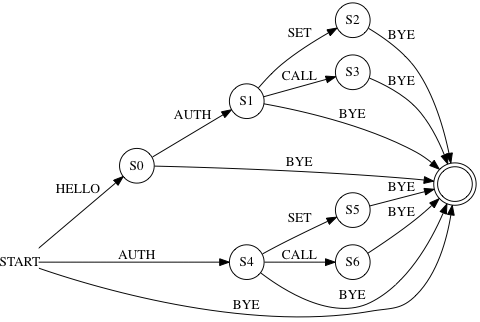
\includegraphics[width=0.5\textwidth]{protocoldiagram}
\label{fig:psm_example}
\end{figure}

An example of a protocol state machine can be seen in Figure \ref{fig:psm_example}.
Since there is no information about the states and their meaning, the states are represented by circles with generic names (e.g. $S0$).
The arrows represent input strings which allow for transition between states.

\section{Evaluation and Results} \label{results}
\subsection{Finding Input, Input Size and Classifying Input}
\tool{} was tested on [NUMBER] closed-source binaries to measure its effectiveness.
The results are summarized in Figure [FIGURE].
Out of the total [NUMBER] binaries, [NUMBER2] had predefined accepted input strings.
\tool{} found 100\% of the input strings for [NUMBER3]...
[CONTINUE].
%To further show the advantage of this method, we built a smart fuzzer which uses our method to determine input and protocol for a given binary.
%We use the smart fuzzer and compare it to black box fuzzers symbolic execution engines with respect to code coverage over units of time.
%Using such a comparison allows the reader to determine which method is more efficient while also performing well.

% 7f... tic tac toe, asks for player names first so without skipping those steps it cannot find any valid input

Additionally, our method was tested on a binary used for technical interviews.
The binary was designed as a reverse engineering challenge for interviewers.
To pass the challenge, the interviewer has to crack the secret passcode to the program.
The blog post describes the manual process used to crack the password \cite{interviewbinary}.
The manual process is tedious and it includes methods such as disassembling the binary, stepping through the instructions using a debugger, and reverse engineering the logic of the program.
As described in the blog post, the cracking of the binary can take several hours and requires advanced skills and years of background knowledge.
\tool{} cracked the binary in a matter of minutes autonomously, proving itself as a useful tool not only finding valid input but also cracking passwords.

\subsection{Protocol State Machine Generation}
% TODO
The evaluation of the protocol state machine generator was also done using the DARPA Cyber Grand Challenge binaries.
However, out of the total of [NUMBER] binaries, only [NUMBER] had an implicit protocol.
Our method was able to generate a correct protocol state machine for [NUMBER]\% of these binaries.

The reason for failure include ...

\subsection{Case Study}
One interesting and noteworthy case study is a binary which implements a simple protocol that lets the user call functions applying root64 and parcour schemes.
The binary is built such that after sending the ``HELLO'' command, the binary will generate an authentication token which is echoed to the user and must be used for the ``AUTH" command.
Without proper authentication, the ``SET" and ``CALL" commands have no effect.
Before generating the protocol state machine, \tool{} analyzed the binary and discovered input strings.
The inputs discovered are: ``HELLO", ``AUTH", ``SET", ``CALL" and ``BYE".
These inputs are the only inputs implemented by the binary's protocol.
The protocol state machine generator not only determined that authentication is necessary but also discovered that a user can properly authenticate themselves with a value of 0 or any special character if they omit the ``HELLO" command (Figure \ref{fig:psm_example}).
This shows that the input finding approach in combination with the protocol state machine generator can help identify potential backdoors or unexpected control flow paths for a given program.

\section{Future Work and Limitations} \label{futurework}
While the method presented in this paper has many advantages, it also has a few limitations.
For certain programs that allow any input, such as an echo server, our method is not any more efficient than a black box fuzzer.
Additionally, our method cannot handle cases in which input is composed of multiple inter-dependent fields, such as when the value of a field determines the length of another field.
Also, \tool{} cannot handle programs which validate input fields out of order or use any safe hashing algorithm for their input validation technique. 
In the future, we would like to apply the input finding technique recursively.
It is easy to imagine programs for which the second input varies based on the value of the first input.
Also, as we've experienced during our evaluation, there exist programs which first request for a username, input which will not have any predefined valid values.
It would be helpful to determine such cases, provide some input and continue the execution of the program, applying the input finding technique once again.
However, there are challenges with this, such as determining when to stop.

With respect to the protocol state machine, currently our method uses the input finding technique to determine valid arguments.
However, the protocol state machine does not currently handle situations in which there are no predefined arguments (e.g. given input ``CREATE'' the arguments could be predefined such as ``dog'' or random such as ``x'').
Ultimately, we would like to generate some random arguments that remain constant for every input string in a given permutation.
Moreover, our current approach is not capable of identifying equivalent states. As seen in Figure \ref{fig:psm_example}, the different authentication paths (use of ``HELLO" vs. omission of ``HELLO") lead to different states when in reality the two states are identical.
Also, our method is based on the assumption that given a number of input strings, the majority of input string permutations are not valid and do not reflect the expected protocol.
There may be cases where this assumption does not hold.
In the future, we would like build onto our current approach for generating protocol state machines. 
First, we want to be able to determine if two states are identical for a more accurate protocol state machine.
Furthermore, we want to determine a better approach for identifying the valid sequence of input strings.
One option would be to monitor other aspects of the program, particularly the \textit{.data}, \text{.bss}, and the heap during the executions.
Changes in these may reflect changes of the state of the program.


\section{Conclusions}
This paper introduces two novel techniques for autonomously generating valid input strings for closed x86 binaries and for generating protocol state machine using the discovered input.
For generating valid input strings, our method exploits the number of instructions executed to infer if a given character is valid for a given index of an input string.
This process allows us to recursively and incrementally craft valid inputs.
To further gain knowledge about the user interaction with the program, we test the program with the inputs generated and construct a protocol state machine which depicts the expected order of the input strings.

We show that our proposed methods are efficient and successful by testing them on [NUMBER] DARPA binaries from the Cyber Grand Challenge \cite{darpacgc}. 
Unlike previous works, our methods do not have any fundamental limitations (such as constraint solvers) and are robust enough to handle even binaries of other formats.

We believe that the our techniques could be applied and used for a number of reasons including building test suites, discovering unwanted or unexpected control flow paths and even finding bugs (when used in combination with a fuzzer).


\bibliographystyle{abbrv}
\bibliography{inputfinder}

\end{document}

